
%NOTE: to be used with \usepackage{subfiles} in the main file.
%Subfiles go in folders which live with the main file.
%Bibliography and preamble go in the main file.

%%%%%%%%%%%%%%%%%%%%%%%% PREAMBLE %%%%%%%%%%%%%%%%%%%%%%%%

\providecommand{\main}{..}

\documentclass[main]{subfiles} %Each instance of `../' elevates one folder to find the main file

\begin{document}

%%%%%%%%%%%%%%%%%%%%%%% DOCUMENT %%%%%%%%%%%%%%%%%%%%%%%

% \tableofcontents % Can be useful to load a TOC while writing

\doublespacing

\schapter{Theoretical aspects}

\hypsection{Jets and algorithms}
\vspace{20pt}

After being produced in a high-energy event, quarks and gluons fragment and hadronize resulting in a collimated spray of hadrons called a jet. The reason behind the process of hadronization lies in the concept of colour confinement. In quantum chromodynamics (QCD), colour confinement states that only objects with non zero colour charge can propagate as free particles, therefore quarks and gluons are only seen bound together in the form of hadrons. When particles carrying colour charge (namely quarks and gluons) are separated in a high-energy event, new colour carrying particles are spontaneously created from the vacuum in order to form colourless hadrons, thus obeying confinement. \\

While hadronization is not yet fully understood and a theoretical description of the process is not yet available, there is a number of phenomenological models such as the Lund String Model that do a good job of describing it \cite{Andersson1983}. The phenomenon can be understood qualitatively through these models by taking into account that the gluon field between colour charges becomes a narrow flux tube as they get separated and eventually it becomes energetically favourable for a new particle to appear rather than extending the tube further, as can be seen in figure \ref{fig:hadronization}.\\

\begin{figure}[h]
    \centering
    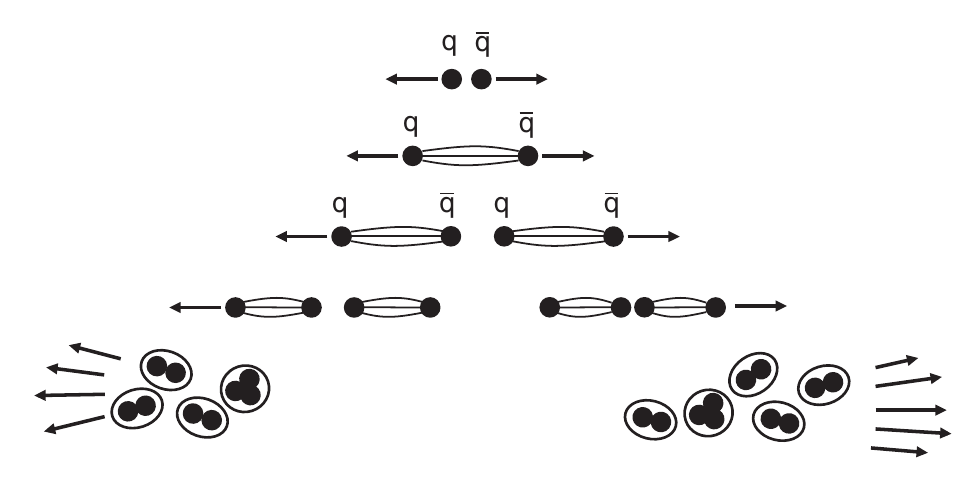
\includegraphics[width=0.8\textwidth]{../Figures/Theory/hadronization.png}
    \caption{Schematic representation of the hadronization process. Image taken from \cite{Thomson2013}.}
    \label{fig:hadronization}
\end{figure}

The particles resulting from the hadronization of a single quark (parton) tend to travel in the same direction as their parent forming a narrow cone, which is what is known as a jet. In particle detector experiments jets are observed instead of quarks, and their structure is quite visible when looking at the events reconstructed in the detector. Through the measurement of the different properties of a jet it is possible to obtain information about the original parton that originated it. Therefore jets are an essential part of the analyses carried out in collider experiments.\\

As important as they are, to be used effectively in analyses jets need to be well defined. As stated in the work of \citet{Salam2010} a jet definition is constituted by a jet algorithm with its respective parameters and recombination scheme. A jet algorithm is a set of rules that group particles into jets. These algorithms usually involve parameters that govern their behaviour, for example in defining how close two particles need to be in order for them to be considered part of the same jet. Jet algorithms are also related to a certain recombination scheme, which indicates how the momentum is assigned to the object resulting of merging two particles during a clustering process.\\

Jet algorithms can be usually classified into two broad categories: cone algorithms and sequential recombination algorithms. Cone algorithms originate from the initial idea of \citet{Sterman1977}. They are considered "top-down" algorithms, since they group together particles within specific conical angular regions so that the resulting cone is "stable", meaning that the direction of the cone matches that of the 4-momenta sum of the particles. On the other hand, sequential recombination algorithms are considered "bottom-up", as they iteratively recombine nearby particles in accordance to a certain distance measure.\\

The anti-$k_t$ algorithm \cite{Cacciari2008} is a sequential recombination algorithm widely used in collider experiments, being also the preferred jet identification algorithm in ATLAS analyses. Since the present study is based on simulated data from this detector (see section \ref{sect:event-generation-chain}) it is relevant to give a brief overview of this algorithm. The anti-$k_t$ takes as an input a list of $N$ objects and it returns a list of jets, which correspond to clusters of said objects grouped according to specific rules regarding distances between them. The distances used by the algorithm are calculated from the quantities $k_{tX}$, $\eta_X$ and $\phi_X$ which correspond to the transverse momentum, pseudo-rapidity and azimuthal angle of the object $X$. These distances are $d_{ij}$ (the distance between objects $i$ and $j$) and $d_{iB}$ (the distance between the object $i$ and the beam), they are defined as follows:
\begin{align}
  d_{ij} &= \text{min}(k_{ti}^{-2},k_{tj}^{-2})\frac{\Delta_{ij}^2}{R^2} \quad ,\\
  d_{iB} &= k_{ti}^{-2} \quad ,
\end{align}
where $\Delta_{ij}^2 = (\eta_i - \eta_j)^2 + (\phi_i - \phi_j)^2$ and $R$ is the radius parameter that sets the size scale of the jets found. The algorithm iteratively forms clusters by identifying the smallest of the two distances for all the objects in the input list. If $d_{ij}$ is the smallest, objects $i$ and $j$ are recombined and replaced in the object list by the recombined object. If on the other hand $d_{iB}$ is the smallest, object $i$ is removed from the object list and marked as a jet.\\

\hypsection{Boosted particles and fat jets}
\label{sect:boosted-particles}
\vspace{20pt}

The use of the term "boosted" in particle physics originates from the concept of a Lorentz boost, which is a type of rotation-free Lorentz transformation between frames moving with different velocities. A "boosted object" refers then to a particle which travels at a very high speed (with very high transverse momentum $p_T$) after being produced in a collision. With the high centre-of-mass energy that has been achieved by the LHC (see section \ref{sect:LHC_ATLAS}) large samples of top quarks, $W$, $Z$ and Higgs bosons with a $p_T$ considerably higher than their rest mass $m$ ($p_T \gg m$) are being produced like never before \cite{Altheimer2014}, which might also be true for heavier particles that remain yet unknown. However, in this kinematic regime the traces left by even well-known particles differ greatly from those left by the same particles with lower $p_T$ values.\\

When a massive particle that has been produced with a significant boost decays hadronically, its decay products appear collimated in the momentum direction of the boosted mother particle. If the particle is boosted enough it won't decay to separated (resolved) jets but into collimated jets which will merge. As a result, what is detected are not multiple jets but a single large R jet, usually called fat jet \cite{Schatzel2015}. The effect of the boost of a particle in its decay is illustrated in figure \ref{fig:boosted_decay}.\\

\begin{figure}[h]
    \centering
    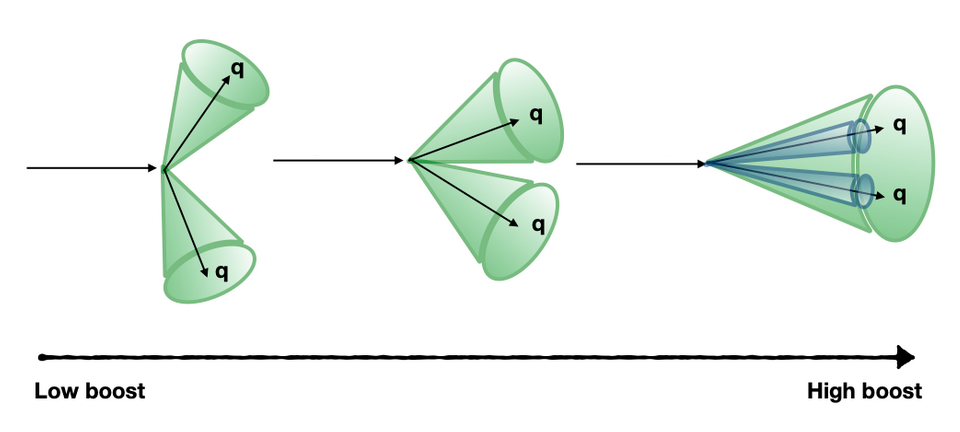
\includegraphics[width=0.8\textwidth]{../Figures/Theory/boosted_decay.png}
    \caption{Schematic representation of jets arising from a particle that decays to two quarks with increasing Lorentz boost. Image taken from \cite{CMSCollaboration2022}.}
    \label{fig:boosted_decay}
\end{figure}

For a two-body decay, the distance between the decay products of a particle in the rapidity-azimuth plane $\left(\Delta R = \sqrt{\eta^2 + \phi^2}\right)$ is given by:
\begin{equation}
  \Delta R \approx \frac{2m}{p_T} \quad ,
\end{equation}
in which $m$ and $p_T$ are the mass and the transverse momentum of the particle. If the $p_T$ of the mother particle is high enough the decay products will be too close for conventional reconstruction techniques to be able to resolve them. As an example, for a $W$ boson with $p_T = 300$\;GeV the distance between its decay products is $\Delta R \approx 0.5$. Reconstructing them with jets of the conventional size used in the LHC ($R = 0.4-0.6$) would result in a failed attempt.\\

The chosen strategy to deal with the hadronic decays of these boosted particles is to use a much larger jet radius parameter in order to capture the energy of the whole decay in a single fat jet. The key to identifying and measuring boosted particles lies then in the internal structure of the reconstructed fat jets \cite{ATLASCollaboration2012}, whose discriminating power is the object of our study. Since it is important that the fat jets contain all of the decay products of the boosted particles, there will be a minimum possible size for the fat jet radius parameter, which will decrease as the boost of the particle increases. An example can be seen in figure \ref{fig:DeltaR_top_decay}, in which the distance between the products in hadronic top quark decay $t \to bqq$ define the minimum radius parameter that should be used for the reconstructed fat jet.\\ 

\begin{figure}[h]
    \centering
    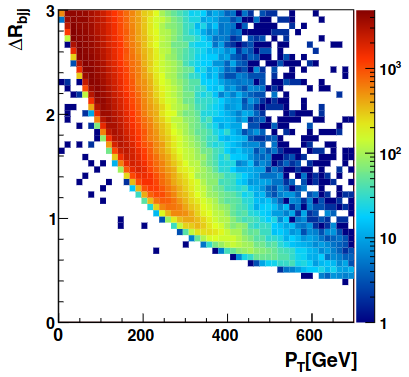
\includegraphics[width=0.5\textwidth]{../Figures/Theory/DeltaR_top_decay.png}
    \caption{Distance between the products of the decay $t \to bqq$ as a function of the top quark $p_T$.  Image taken from \cite{Plehn2010}.}
    \label{fig:DeltaR_top_decay}
\end{figure}

\pagebreak

\hypsection{Fat jet substructure: N-subjettiness}
\label{sect:substructure}
\vspace{20pt}

The high centre-of-mass energy achieved by the LHC together with the detection capabilities of the ATLAS calorimeter provide an excellent environment to study hadronic jets. Analyses involving hadronic decay channels are becoming increasingly more relevant after it was initially shown that these channels become usable by looking at boosted topologies \cite{Butterworth2008}. Hadronic channels often have the highest branching ratios, but had been considered impractical due to the large background they present at a hadron collider.\\

The efficient reconstruction and identification of boosted object decays is of utmost importance in searches of new phenomena at high energies. As was stated in the end of section \ref{sect:boosted-particles}, the internal structure of fat jets give us crucial information for the identification of boosted particles. Therefore, since the utility of boosted signals was brought to light, several studies on jet substructure have been carried out \cite{Behr2014} and a rich and continuously expanding field was born. The objective of these studies is to increase how well the jets resulting from boosted electroweak bosons and top quarks can be distinguished from background QCD jets (originating from hard light quarks or gluons).\\

Substructure information used to distinguish between jets originating from boosted hadronically decaying objects and QCD jets is extracted from the jet clustering procedure by algorithmic methods called shape methods. Jet shape methods use certain observables that take advantage of the different energy flow in the decay pattern of signal and background jets. The method studied in this work revolves around a group of variables called $N$-subjettiness, a jet shape denoted by $\tau_N$ and first introduced by \citet{Thaler2011}, which is based on the original $N$-jettiness shape \cite{Stewart2010}.\\

The energy pattern of boosted hadronically decaying particles is fundamentally different from that of QCD jets of a similar invariant mass. As an example, take the case of a boosted $W$ boson (a similar discussion holds for the case of other boosted objects), which decays hadronically to two quarks. The single jet containing the decay products of the boosted $W$ should be composed of two distinct subjets with a combined invariant mass near 80\;GeV. A background QCD fat jet with a similar invariant mass originates from a single hard parton and acquires mass through large angle soft splittings. $N$-subjettiness exploits the difference in energy flow between this two types of jet by taking into account the number of energy lobes within each one. This difference can be easily seen in the reconstructed jets for the previous example, as shown in figure \ref{fig:energyflow_W_QCD}.\\

\begin{figure}[h]
     \centering
     \begin{subfigure}[h]{\textwidth}
         \centering
         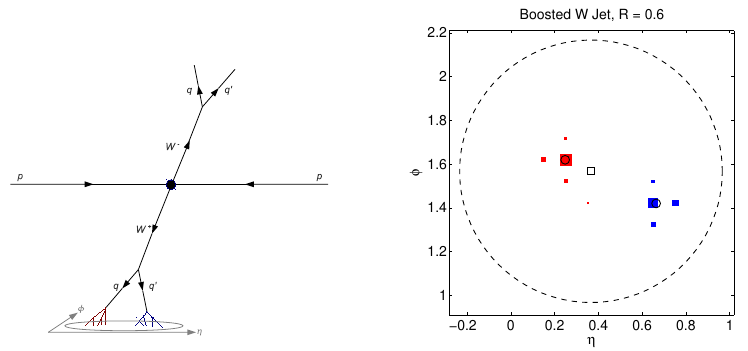
\includegraphics[width=0.8\textwidth]{../Figures/Theory/eflow_W.png}
         \caption{}
         \label{fig:eflow_W}
     \end{subfigure}
     \hfill
     \begin{subfigure}[h]{\textwidth}
         \centering
         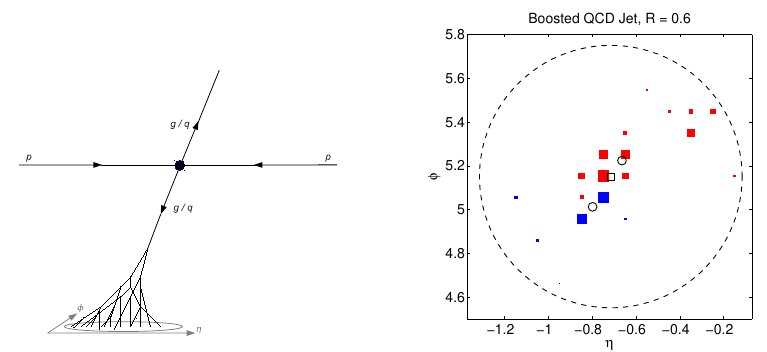
\includegraphics[width=0.8\textwidth]{../Figures/Theory/eflow_QCD.png}
         \caption{}
         \label{fig:eflow_QCD}
     \end{subfigure}
     \caption{Schematic of the hadronic decay and a typical event display for a reconstructed jet with mass $m \approx$ 80\;GeV in (a) $W^+W^-$ and (b) dijet QCD events. The jets are clustered with the anti-$k_T$ algorithm using $R = 0.6$. The marker size for each calorimeter cell is proportional to the logarithm of the energy deposition and each marker color corresponds to a subjet found by the anti-$k_T$. The small square indicates the total jet direction and the small circles the two subjet directions. Image taken from \cite{Thaler2011}.}
        \label{fig:energyflow_W_QCD}
\end{figure}

The $N$-subjettiness jet shape denoted by $\tau_N$ is defined using the $N$ candidate subjets identified during the jet clustering process as follows:
\begin{equation}
  \tau_N = \frac{1}{d_0}\sum_k p_{T,k} \times \text{min}(\Delta R_{1,k},\Delta R_{2,k},\dots,\Delta R_{N,k}) \quad ,
\end{equation}
where $k$ runs over the constituent particles of the jet, $p_{T,k}$ is their transverse momenta, $\Delta R_{i,k}$ is the distance in the rapidity-azimuth plane between the candidate subjet $i$ and the constituent particle $k$, and $d_0$ is a normalization factor taken as:
\begin{equation}
  d_0 = \sum_k p_{T,k} R_0 \quad ,
\end{equation}
where $R_0$ is the jet radius parameter used in the original jet clustering algorithm.\\

As can be seen from its definition, $\tau_N$ gives us information about how well the jet substructure is described by $N$ subjets, or in other words, how "$N$-subjetty" the jet is. This is done by assessing the degree to which constituent particles are near the subjets. A jet with $\tau_N \approx 0$ has most of its radiation aligned with the direction of the candidate subjets and therefore tends to have $N$ (or fewer) subjets.\\

A jet originating from a boosted $W$ is expected to have a small $\tau_2$ value. However, QCD jets can also have small $\tau_2$ values. Likewise, $W$ jets are expected to have large $\tau_1$, but QCD jets can also have large $\tau_1$. The key to using $N$-subjettiness as a discriminating variable effectively lies in the fact that QCD jets with large $\tau_1$, which correspond to jets with a diffuse spray of large angle radiation, typically have large $\tau_2$ values as well. Therefore, the preferred discriminating variable will be the ratio $\tau_2 / \tau_1$ usually denoted as $\tau_{21}$ \cite{Thaler2012}.\\

It should be noted that the previous discussion holds for boosted $Z$ bosons and Higgs bosons as well. In the case of boosted top quarks, the decay chain needs to be taken into account. Fully hadronically decaying top quarks decay to a $b$ jet and a $W$ boson, followed by the decay of the $W$ boson to two quarks. Therefore a jet resulting from a boosted top quark will have three lobes of energy, not two. Thus, the preferred discriminating variable for top quarks will be $\tau_{32}$ instead of $\tau_{21}$.\\

Finally, it is important to clarify how jet mass is defined, since it will be used together with the $N$-subjettiness as it is a variable with discriminating power (on its own). Jet mass $M$ is calculated from the energies and momenta of its constituents as follows:
\begin{equation}
  M^2 =  \left(\sum_i E_i\right)^2 + \left(\sum_i \vec{p}_i\right)^2 \quad ,
\end{equation}
where $E_i$ and $\vec{p}_i$ are the energy and three-momentum of the $i^{th}$ constituent.\\

\hypsection{The LHC and the ATLAS detector}
\label{sect:LHC_ATLAS}
\vspace{20pt}

The Large Hadron Collider (LHC) \cite{Evans2008} is the world's largest particle accelerator. It was built by the European Organization for Nuclear Research (CERN) in the existing 26.7\;km tunnel that was constructed originally for the Large Electron-Positron Collider (LEP), which lies between 50\;m and 175\;m below the surface beneath the France-Switzerland border. The 3.8\;m wide tunnel contains two adjacent beamlines, which allow two high-energy particle beams to travel in opposite directions around the accelerator ring. The beams are guided by about 10.000 superconducting magnets \cite{MYERS2013}, dipole magnets are used to bend the beams, quadrupole magnets are used to focus them and magnets of higher multipole orders are used for smaller corrections in the geometry of the field.\\

The maximum energy that can be reached by the protons in the beam is limited by the peak dipole field, which has a nominal value of 8.33\;T (corresponding to a proton energy of 7\;TeV) \cite{Bruning2004}. However, the actual value of the attainable field depends on external factors that cause beam losses. As such, the highest proton energy achieved as of today is 6.8\;TeV, which in turn means an attained centre-of-mass energy of $\sqrt{s} = $13\;TeV. In order to achieve said energy, before being injected to the LHC the protons are pre-accelerated in a series of steps in which their energy is successively increased (see figure \ref{fig:preaccelerators}). Initially, H$^-$ ions with an energy of 160\;MeV are produced in the linear accelerator LINAC4, which feeds the Proton Synchrotron Booster (PSB), where the electrons are stripped from the ions and the remaining protons are accelerated to 2\;GeV and injected into the Proton Synchrotron (PS), which accelerates them to 26\;GeV and injects them into the Super Proton Synchrotron (SPS) where they are accelerated to 450\;GeV before being finally injected into the main ring.\\

\begin{figure}[h]
    \centering
    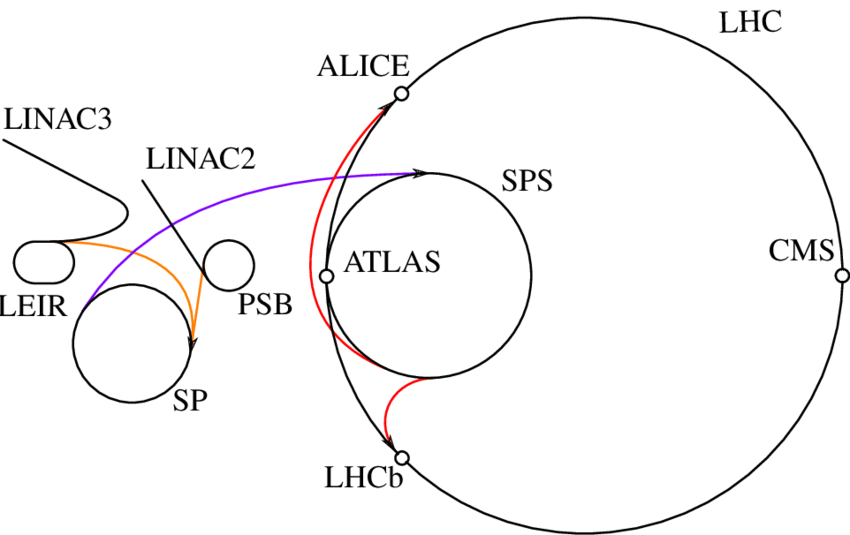
\includegraphics[width=0.8\textwidth]{../Figures/Theory/LHC_preaccelerators.png}
    \caption{Schematic representation of the LHC and its pre-accelerators (in 2020 LINAC2 was replaced by LINAC4). Image taken from \cite{Michael2011}.}
    \label{fig:preaccelerators}
\end{figure}

It is also worth noting that the protons do not travel in the form of continuous beams, but rather in bunches of 10$^{11}$ protons each. Under nominal operating conditions each proton beam is composed of 2808 bunches, so that interactions take place at discrete intervals each 25\;ns (collision rate of 40\;Hz). Taking into account the previous parameters the design (proton-proton) luminosity of the LHC is 10$^{34}$\;cm$^{-2}$s$^{-1}$.\\ 

The two beams intersect at four different points around the accelerator ring, which is where the collisions occur. Specially strong magnets are used near these points in order to increase the interaction chance. Built around the collision points are seven experiments installed in underground caverns \cite{Lopes2022}. Of these, the main four are the ATLAS, CMS, LHCb and ALICE detectors. These detectors are used to count, track and characterize all the particles that are produced in the collisions in order to reconstruct the different events as a whole. As was stated previously, this study will be carried out using simulated data from ATLAS, therefore an overview of the detector will be given below.\\

The ATLAS (A Toroidal LHC ApparatuS) detector \cite{Aad2008} is a multi-purpose detector designed to cover a wide range of physics at the LHC. The detector is forward-backward symmetric with respect to the interaction point, and it has nearly full coverage in solid angle. In order to reconstruct the particles originated from the collisions, ATLAS is composed of multiple layers, each one of them sensitive to different types of particles. The detector layout is shown in figure \ref{fig:ATLAS_detector}.\\

\begin{figure}[h]
    \centering
    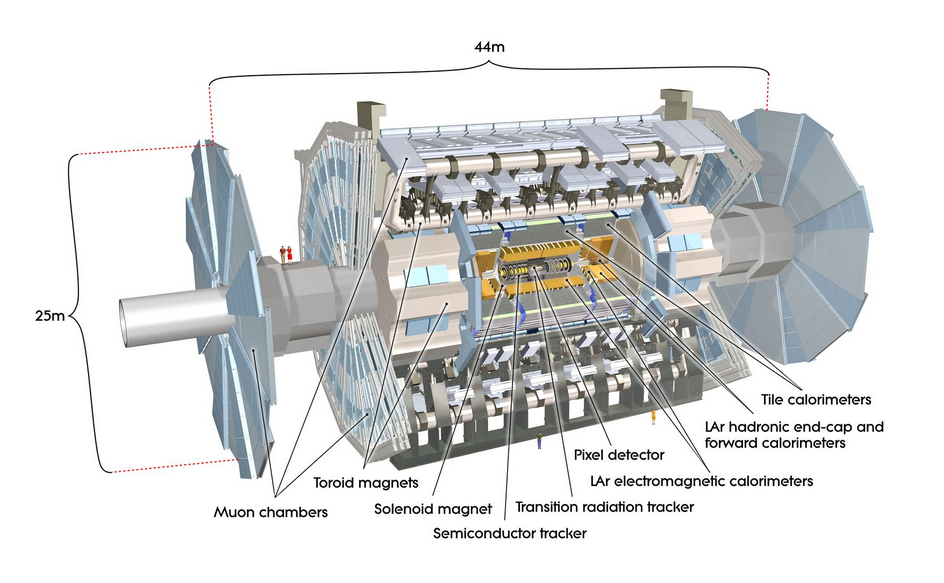
\includegraphics[width=0.8\textwidth]{../Figures/Theory/ATLAS_detector.png}
    \caption{Cut-away view of the ATLAS detector. Image taken from \cite{Aad2008}.}
    \label{fig:ATLAS_detector}
\end{figure}

The layers \cite{Airapetian1999} that are closer to the interaction point form what is known as the inner detector, they are immersed in a 2\;T magnetic field generated by a solenoid magnet. Charged particles are curved by this field and their trajectories (tracks) are measured by silicon pixel and microstrip detectors, which are surrounded by a transition radiation tracker. Surrounding the inner detector is the calorimeter system, composed by the liquid argon (LAr) electromagnetic calorimeters and the scintillator-tile hadronic calorimeters. LAr technology is also used in the hadronic end-caps (matching the outer limits of the electromagnetic calorimeters) and forward calorimeters, which extend the detection coverage. Both the electromagnetic and hadronic calorimeters use the same principle: when a particle enters the calorimeter, it showers and deposits energy in the calorimeter cells. The difference between the two kind of calorimeters lies in the materials they are made of and the size of the cells, which determine the particles they target (electromagnetic calorimeters targeting electrons and photons and hadronic calorimeters targeting hadrons). Surrounding the calorimeter system is the muon spectrometer, which is designed to measure the muon tracks (together with neutrinos, muons are the only particles not stopped by the calorimeters). It is composed of high precision tracking chambers immersed in a magnetic field provided by toroid magnets.\\

\hypsection{Event generators}
\vspace{20pt}



















% \bibliographystyle{../../PhilReview} %%bib style found in bst folder, in bibtex folder, in texmf folder.
% \nobibliography{Zotero} %%bib database found in bib folder, in bibtex folder
% \nobibliography{../../Thesis_bib}
\biblio

\end{document}
